\hypertarget{_style_8h}{
\section{Style.h File Reference}
\label{_style_8h}\index{Style.h(111)@{Style.h(111)}}
}


\subsection{Detailed Description}
Declaration of class \hyperlink{class_style}{Style}. 



Definition in file \hyperlink{_style_8h-source}{Style.h}.

{\tt \#include \char`\"{}FontWeight.h\char`\"{}}\par
{\tt \#include \char`\"{}RgbColor.h\char`\"{}}\par


Include dependency graph for Style.h:\nopagebreak
\begin{figure}[H]
\begin{center}
\leavevmode
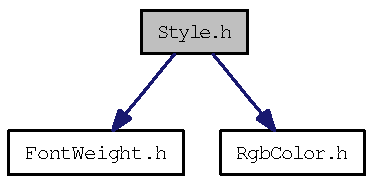
\includegraphics[width=107pt]{_style_8h__incl}
\end{center}
\end{figure}


This graph shows which files directly or indirectly include this file:\nopagebreak
\begin{figure}[H]
\begin{center}
\leavevmode
\includegraphics[width=159pt]{_style_8h__dep__incl}
\end{center}
\end{figure}
\subsection*{Data Structures}
\begin{CompactItemize}
\item 
class \hyperlink{class_style}{Style}
\begin{CompactList}\small\item\em Font style of a character. \item\end{CompactList}\end{CompactItemize}
